%%%%%%%%%%%%%%%%%%%%%%%%%%%%%%%%%%%%%%%%%%%%%%%%%%%%%%%%%%%%%%%%%%%%%%%%%%%%%%%%%
\subsection{Low-Order Scheme}
%%%%%%%%%%%%%%%%%%%%%%%%%%%%%%%%%%%%%%%%%%%%%%%%%%%%%%%%%%%%%%%%%%%%%%%%%%%%%%%%%
\begin{frame}
\frametitle{Low-Order Scheme}

\begin{itemize}
   \item To get the low-order scheme, one does the following:
   \begin{itemize}
      \item Lumps the mass matrix:
        $\consistentmassmatrix\rightarrow\lumpedmassmatrix$.
      \item Adds a low-order diffusion operator:
        $\ssmatrix \rightarrow \ssmatrix+\loworderdiffusionmatrix$.
   \end{itemize}
   \item This gives the following, where $\solutionvector^{L,n+1}$ is the
     low-order solution:
   \begin{equation}
      \textcolor{secondarycolorheavy}{\lumpedmassmatrix}
        \frac{\solutionvector^{L,n+1}-\solutionvector^n}{\dt}
        + (\ssmatrix + \textcolor{secondarycolorheavy}{\diffusionmatrix^L})
          \solutionvector^n = \ssrhs^n \eqp
   \end{equation}
   \item The diffusion matrix $\diffusionmatrix^L$ is assembled elementwise,
      where $K$ denotes an element, using a local bilinear form $b_K$ and a
      local low-order viscosity $\nu_K^L$:
   \begin{equation}
      D\ij^L = \sumKSij \nu_K^L b_K(\testfunction_j,\testfunction_i) \eqp
   \end{equation}
\end{itemize}

\end{frame}
%%%%%%%%%%%%%%%%%%%%%%%%%%%%%%%%%%%%%%%%%%%%%%%%%%%%%%%%%%%%%%%%%%%%%%%%%%%%%%%%%
\begin{frame}
\frametitle{Local Viscous Bilinear Form}

\begin{itemize}
   \item The local viscous bilinear form is defined as follows, where $V_K$ denotes
      the volume of element $K$:
   \begin{equation}
      b_K(\testfunction_j, \testfunction_i) \equiv \left\{\begin{array}{l l}
         -\frac{1}{n_K - 1}V_K & i\ne j, \quad i,j\in \mathcal{I}(K)\\
         V_K                   & i = j,  \quad i,j\in \mathcal{I}(K)\\
         0                & i\notin\mathcal{I}(K)\,|\, j\notin\mathcal{I}(K)
      \end{array}\right. \eqp
   \end{equation}
   \item Some properties that result from this definition are
   \begin{subequations}
   \begin{equation}
      b_K(\testfunction_i, \testfunction_i) > 0 \eqp
   \end{equation}
   \begin{equation}
      b_K(\testfunction_j, \testfunction_i) < 0 \quad j \ne i \eqp
   \end{equation}
   \begin{equation}
      \sum\limits_j b_K(\testfunction_j, \testfunction_i) = 0 \eqp
   \end{equation}
   \end{subequations}
  \item The local viscous matrix in 1-D is
    \begin{equation}
      \mathbf{D}_K = \left[\begin{array}{r r}
           1 & -1\\
          -1 &  1
        \end{array}\right]\Delta x_K \eqp
    \end{equation}
\end{itemize}

\end{frame}
%%%%%%%%%%%%%%%%%%%%%%%%%%%%%%%%%%%%%%%%%%%%%%%%%%%%%%%%%%%%%%%%%%%%%%%%%%%%%%%%%
\begin{frame}
\frametitle{Low-Order Viscosity}

\begin{itemize}
   \item The low-order viscosity is defined as
   \begin{equation}
     \lowordercellviscosity[\timeindex] \equiv \max\limits_{i\ne j\in\indices(\cell)}
     \frac{\max(0,\ssmatrixletter\ij^\timeindex)}
     {-\mkern-20mu\sumKSij[T]\mkern-20mu\localviscbilinearform{T}{j}{i}}
     \eqp
   \end{equation}
   \item This definition is designed to be the smallest number such that the
      following is guaranteed:
   \begin{equation}
      D^L\ij \leq -A\ij, \quad j\ne i \eqp
   \end{equation}
   \item This is used to guarantee that the low-order steady-state matrix
      $\ssmatrix^L=\ssmatrix+\diffusionmatrix^L$ is an M-matrix.
\end{itemize}

\end{frame}
%%%%%%%%%%%%%%%%%%%%%%%%%%%%%%%%%%%%%%%%%%%%%%%%%%%%%%%%%%%%%%%%%%%%%%%%%%%%%%%%%
\begin{frame}
\frametitle{M-Matrix Property}

\begin{itemize}
  \item An M-matrix, also known as a \hlorange{monotone matrix}, or
    \hlorange{inverse-positive matrix} has the property
    \begin{equation}
      \mathbf{A}\mathbf{x}=\mathbf{b} \ge 0\Rightarrow \mathbf{x}\ge 0 \eqp
    \end{equation}
  \item Therefore one can prove \hlorange{non-negativity} of the solution of
    a linear system $\mathbf{A}\solutionvector=\mathbf{b}$ by proving that
    $\mathbf{A}$ is an M-matrix and $\mathbf{b}$ is non-negative.
  \item An M-matrix can be identified by verifying the following properties:
    \begin{subequations}
      \begin{equation}
        A\ij \leq 0 \quad j \ne i \quad \forall i
      \end{equation}
      \begin{equation}
        A_{i,i} \geq 0 \quad \forall i
      \end{equation}
      \begin{equation}
        \sumj A\ij \geq 0 \quad \forall i
      \end{equation}
    \end{subequations}
\end{itemize}

\end{frame}
%%%%%%%%%%%%%%%%%%%%%%%%%%%%%%%%%%%%%%%%%%%%%%%%%%%%%%%%%%%%%%%%%%%%%%%%%%%%%%%%%
\begin{frame}
\frametitle{Local Discrete Maximum Principle for Explicit Euler}

\begin{itemize}
  \item If the following CFL-like condition is satisfied:
    \begin{equation}
      \dt \leq \frac{\massmatrixletter^L_{i,i}}{
        \ssmatrixletter_{i,i}^{L}}
      \quad\forall i \eqc
    \end{equation}
  then the low-order solution for explicit Euler satisfies the following
  \hlorange{local discrete maximum principle} (DMP):
      \begin{subequations}
      \begin{equation}
         \DMPlowerbound_i \leq
         U_i^{L,n+1}\leq
         \DMPupperbound_i \qquad\forall i \eqc
      \end{equation}
      \begin{equation}
         \DMPbounds_i \equiv U_{\substack{\max\\\min},i}^n\left(
         1-\frac{\dt}{M_{i,i}^L}
         \sum\limits_j A\ij^L\right)
         + \frac{\Delta t}{M_{i,i}^L}b_i^n \eqc
      \end{equation}
      \begin{equation}
        U^n_{\substack{\max\\\min},i}
          = \substack{\max\\\min\limits_{j\in\mathcal{I}(S_i)}} U^n_j \eqp
      \end{equation}
      \end{subequations}
%   \item For example, when there is no reaction term or source term, this reduces
%      to the following DMP, which implies the scheme is local extremum
%      diminishing (LED):
%      \begin{equation}
%         U^n_{\min,i}\leq
%         U_i^{L,n+1}\leq
%         U^n_{\max,i}\qquad\forall i \eqp
%      \end{equation}
\end{itemize}

\end{frame}
%%%%%%%%%%%%%%%%%%%%%%%%%%%%%%%%%%%%%%%%%%%%%%%%%%%%%%%%%%%%%%%%%%%%%%%%%%%%%%%%%
\begin{frame}
\frametitle{Local Discrete Maximum Principle for Theta Method}

\begin{itemize}
  \item If the following CFL-like condition is satisfied:
    \begin{equation}
      \dt \leq \frac{\massmatrixletter^L_{i,i}}{(1-\theta)
        \ssmatrixletter_{i,i}^{L}}
      \quad\forall i \eqc
    \end{equation}
   then the low-order theta method solution satisfies the following local DMP,
   which is \hlorange{implicit}:
\begin{subequations}
\begin{multline}
   \DMPbounds_i\hlorange{(\solutionvector^{L,n+1})}
   \equiv
   \frac{1}{1+\frac{\theta\timestepsize}{\massmatrixletter^L_{i,i}}
       \ssmatrixletter_{i,i}^{L}}
     \Bigg[\pr{1 - \frac{(1-\theta)\timestepsize}{\massmatrixletter^L_{i,i}}
     \ssmatrixletter_{i,i}^{L}}\solutionletter_i^\timeindex
     \\
     - \frac{\timestepsize}{\massmatrixletter^L_{i,i}}
       \sumjnoti\ssmatrixletter_{i,j}^{L}\pr{
         (1-\theta)\solutionletter_{\substack{\max\\\min},j\ne i}^n
         + \theta\hlorange{\solutionletter_{\substack{\max\\\min},j\ne i}^{L,n+1}}}
     + \frac{\timestepsize}{\massmatrixletter^L_{i,i}}
       \ssrhsletter_i^\theta\Bigg] \eqc
\end{multline}
\begin{equation}
  \solutionletter_{\substack{\max\\\min},j\ne i}^\timeindex
  \equiv \substack{\max\\\min\limits_{j\ne i\in\indices(\support_i)}}
    \solutionletter_j^\timeindex
  \eqp
\end{equation}
\end{subequations}
\end{itemize}

\end{frame}
%%%%%%%%%%%%%%%%%%%%%%%%%%%%%%%%%%%%%%%%%%%%%%%%%%%%%%%%%%%%%%%%%%%%%%%%%%%%%%%%%
\begin{frame}
\frametitle{Low-Order Scheme Results Example}
\framesubtitle{Linear Advection of Discontinuous Wave Front}

\begin{center}
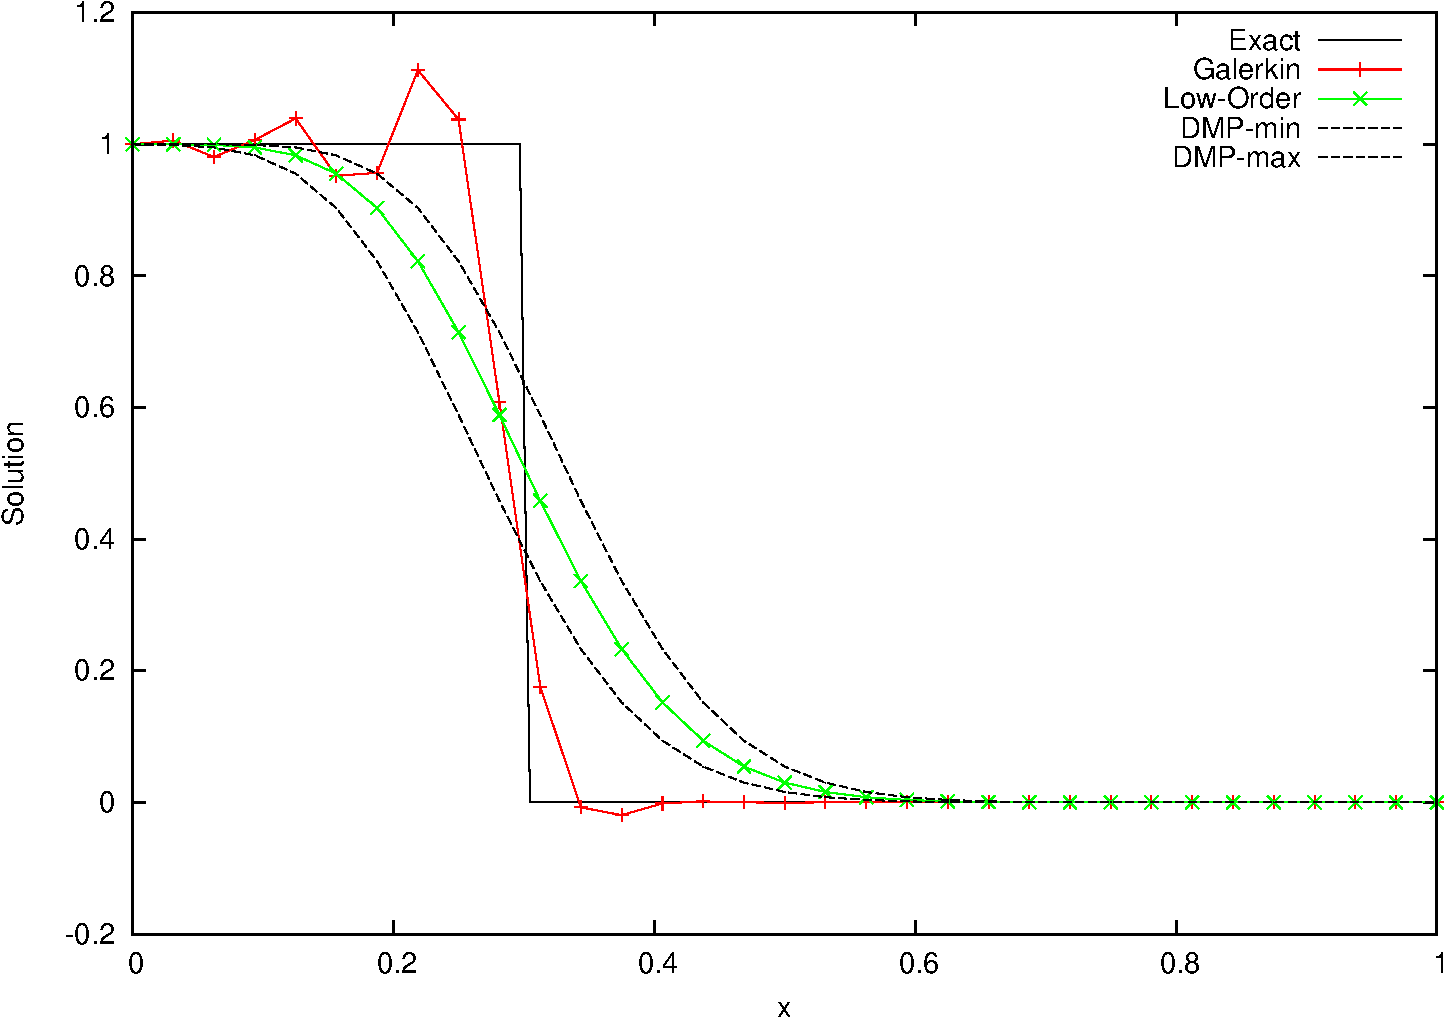
\includegraphics[width=0.85\textwidth]{./figures/advection_low_order.pdf}
\end{center}

\end{frame}
